\documentclass[digital, oneside, table, nolot, nolof]{fithesis3}
%\documentclass[printed, twoside, table, nolot, nolof]{fithesis3}

%% The following section sets up the locales used in the thesis.
\usepackage[resetfonts]{cmap}
\usepackage[T1]{fontenc}
\usepackage[main=czech, english]{babel}

%% The following section sets up the metadata of the thesis.
\thesissetup{
    date          = \the\year/\the\month/\the\day,
    university    = mu,
    faculty       = fi,
    type          = mgr,
    author        = Jan Horáček,
    gender        = m,
    advisor       = {RNDr. Zdeněk Matěj, Ph.D.},
    title         = {Návrh a implementace nového protokolu sběrnice MTBbus},
    TeXtitle      = {Návrh a implementace nového protokolu sběrnice MTBbus},
    keywords      = {sběrnice, mtb, rs485, embedded, stm32, C++, qt, protokol, avr, arm, kicad},
    TeXkeywords   = {sběrnice, mtb, rs485, embedded, stm32, C++, qt, protokol, avr, arm, kicad},
    abstract      = {Se zaváděním počítačového řízení železniční dopravy vznikaly systémy umožňující
centrálnímu řídicímu počítači interakci s~venkovními prvky zabezpečovacího
zařízení – výhybkami, návěstidly apod. Tato práce se zaměřuje na návrh
a~implementaci sběrnice, která takovou interakci umožní, ovšem na kolejištích
modelových. Práce navrhuje a~implementuje nový protokol sběrnice pro řízení
modelových kolejišť \textit{MTBbus}. Je popsáno, proč je současný systém řízení
kolejiště nedostatečný, jsou formulovány požadavky na nový systém, tento systém
je implementován. V~rámci práce vznikl detailní návrh nového protokolu, nové
hardwarové moduly pro řízení kolejiště, modul pro komunikaci s~počítačem,
obslužný počítačový software a~knihovna integrující nový hardwarový systém se
současným řídicím softwarem kolejiště.  Nový řídicí systém byl otestován
a~nasazen na skutečná kolejiště, čímž umožnil jejich další rozšiřování
a~zprovoznění nových způsobů řízení dopravy. Vznikl otevřený a~robustní systém
s~výhledem dlouhodobé udržitelnosti, který svými vlastnostmi převyšuje mnohé
současné komerční systémy řízení modelových kolejišť.  Vzniknuvší systém je
obecný, takže jej lze použít i~v~mnoha jiných aplikacích.
},
    thanks        = {Děkuji především všem, kteří ve mně zažehli, podporovali a~podporují můj velký
koníček – řízení modelové železnice. Ať už se jedná o~tátu
Miroslava, přítelkyni Verču, členy brněnského modelářského klubu nebo vedoucího
mé diplomové práce Zdeňka Matěje. Všichni ti mi umožnili psát diplomovou práci,
jejíž náplň mi dává smysl, jejíž realizace mě baví a jejíž výsledky vidím
v~reálném světě. Moc si vaší podpory vážím.
Děkuji svému vedoucímu Zdeňku Matějovi za korektury a~podporu ve změně tématu.
Děkuji konzultantovi Honzu Mrázkovi za odpovídání na mé dotazy a~za rady.
Děkuji všem korektorům této práce: Veronice Burgerové, Miroslavu Horáčkovi
a~Zdeňku Matějovi.
Děkuji mé přítelkyni Veronice a tučňákovi Adalbertovi za mentální podporu.
},
    bib           = bibliography.bib,
    titleEn       = {Design and implementation of a new MTBbus protocol},
    TeXtitleEn    = {Design and implementation of a new MTBbus protocol},
    keywordsEn    = {bus, mtb, rs485, embedded, stm32, C++, qt, protocol, avr, arm, kicad},
    TeXkeywordsEn = {bus, mtb, rs485, embedded, stm32, C++, qt, protocol, avr, arm, kicad},
    assignment    = {data/zadani_ofic.pdf},
}
\usepackage{makeidx}      %% The `makeidx` package contains
\makeindex                %% helper commands for index typesetting.
%% These additional packages are used within the document:
\usepackage{paralist} %% Compact list environments
\usepackage{amsmath}  %% Mathematics
\usepackage{amsthm}
\usepackage{amsfonts}
\usepackage{url}      %% Hyperlinks
\usepackage{listings} %% Source code highlighting
\usepackage{enumitem}
\usepackage{afterpage}
\usepackage{glossaries}
\makeglossaries
\lstset{
  basicstyle      = \ttfamily,%
  identifierstyle = \color{black},%
  keywordstyle    = \color{blue},%
  keywordstyle    = {[2]\color{cyan}},%
  keywordstyle    = {[3]\color{olive}},%
  stringstyle     = \color{teal},%
  commentstyle    = \itshape\color{magenta}}
\usepackage{floatrow} %% Putting captions above tables
\floatsetup[table]{capposition=top}
\Urlmuskip=0mu plus 1mu
\begin{document}

% Highlight overfulls
% \setlength{\overfullrule}{5pt} % TODO: remove

\setlength{\parindent}{0cm}
\setlength{\parskip}{3mm plus2pt minus2pt}
\setlist{leftmargin=8mm}
\renewenvironment{compactenum}
	{\begin{enumerate}[leftmargin=8mm,itemsep=0pt,parsep=1pt,topsep=1pt,partopsep=1pt]}
	{\end{enumerate}}
\renewenvironment{compactitem}
	{\begin{itemize}[leftmargin=8mm,itemsep=0pt,parsep=0pt,topsep=1pt,partopsep=1pt]}
	{\end{itemize}}

\newglossaryentry{plc} {
	name=PLC,
	description={Programmable Logic Controller, robustní zařízení průmyslové
	atumatizace}
}

\newglossaryentry{mtb} {
	name=MTB,
	description={Hardwarový systém pro řízení modelových kolejišť složený ze
	sběrnice MTBbus, MTB modulů a~MTB-USB desky}
}

\newglossaryentry{mtbbus} {
	name=MTBbus,
	description={Model Train Bus\footnote{Expanze zkratky do jejího plného
	významu nedává smysl, i tak budeme používat označení MTBbus, protože tak je
	zkratka zaužívaná.}, sběrnice určená pro řízení modelových kolejišť}
}

\newglossaryentry{dcc} {
	name=DCC,
	description={Digital Command Control, mezinárodně užívaný standardizovaný
	systém pro digitální řízení modelové železnice}
}

\newglossaryentry{kmz}{
	name={KMŽ Brno~I},
	description={Klub modelářů železnic Brno~I}
}

\newglossaryentry{nmra}{
	name={NMRA},
	description={National Model Railroad Association}
}

\newglossaryentry{mtbusb}{
	name={MTB-USB},
	description={Master modul sběrnice MTBbus, implementuje rozhraní mezi MTBbus
	a počítačem (USB)}
}

\newglossaryentry{mtbuni}{
	name={MTB-UNI},
	description={Nejrozšířenější slave modul sběrnice MTBbus, má 16~digitálních
	vstupů a~16~digitálních výstupů}
}

\newglossaryentry{ttl}{
	name={TTL},
	description={Transistor-transistor-logic, v~kontextu této práce standard
		definující jaká napěťová úroveň odpovídá jaké logické úrovni}
}

\newglossaryentry{usb}{
	name={USB},
	description={Universal Serial Bus, v současnosti nejpoužívanější sběrnice
	pro připojení periferií k počítači}
}

\newglossaryentry{cdc}{
	name={CDC},
	description={USB Comunications Device Class, třída USB protokolu implementující
		tunelování sériové linky skrze USB}
}

\newglossaryentry{dps}{
	name={dps},
	description={Deska plošnýcn spojů}
}

\printglossary[title=Seznam použitých zkratek]



\chapter{Úvod} \label{chap:uvod}
\textit{Programmable Logic Controller} (\gls{plc}) je vestavěný počítač, který
zpracovává vstupy, provádí jejich vyhodnocování, komunikuje s~dalšími \gls{plc}
obvody a~nastavuje výstupy \cite{plc:web}. Na rozdíl od běžných počítačů typu
\textit{PC} mají \gls{plc} větší množství vstupů a~výstupů, běží na nich
\textit{realtime} operační systémy a~jsou vysoce robustní.

\gls{plc} jsou základní jednotkou průmyslové automatizace. Používají se
například pro řízení světel dopravních křižovatek, výrobních linek, eskálátorů,
řízení elektráren, rozvoden apod. Všude tam \gls{plc} zpracovávají data z~čidel
a~ovládají periferie – například motorické pohony, signalizační diody,
robotické ruky, lasery apod.

\begin{figure}[ht]
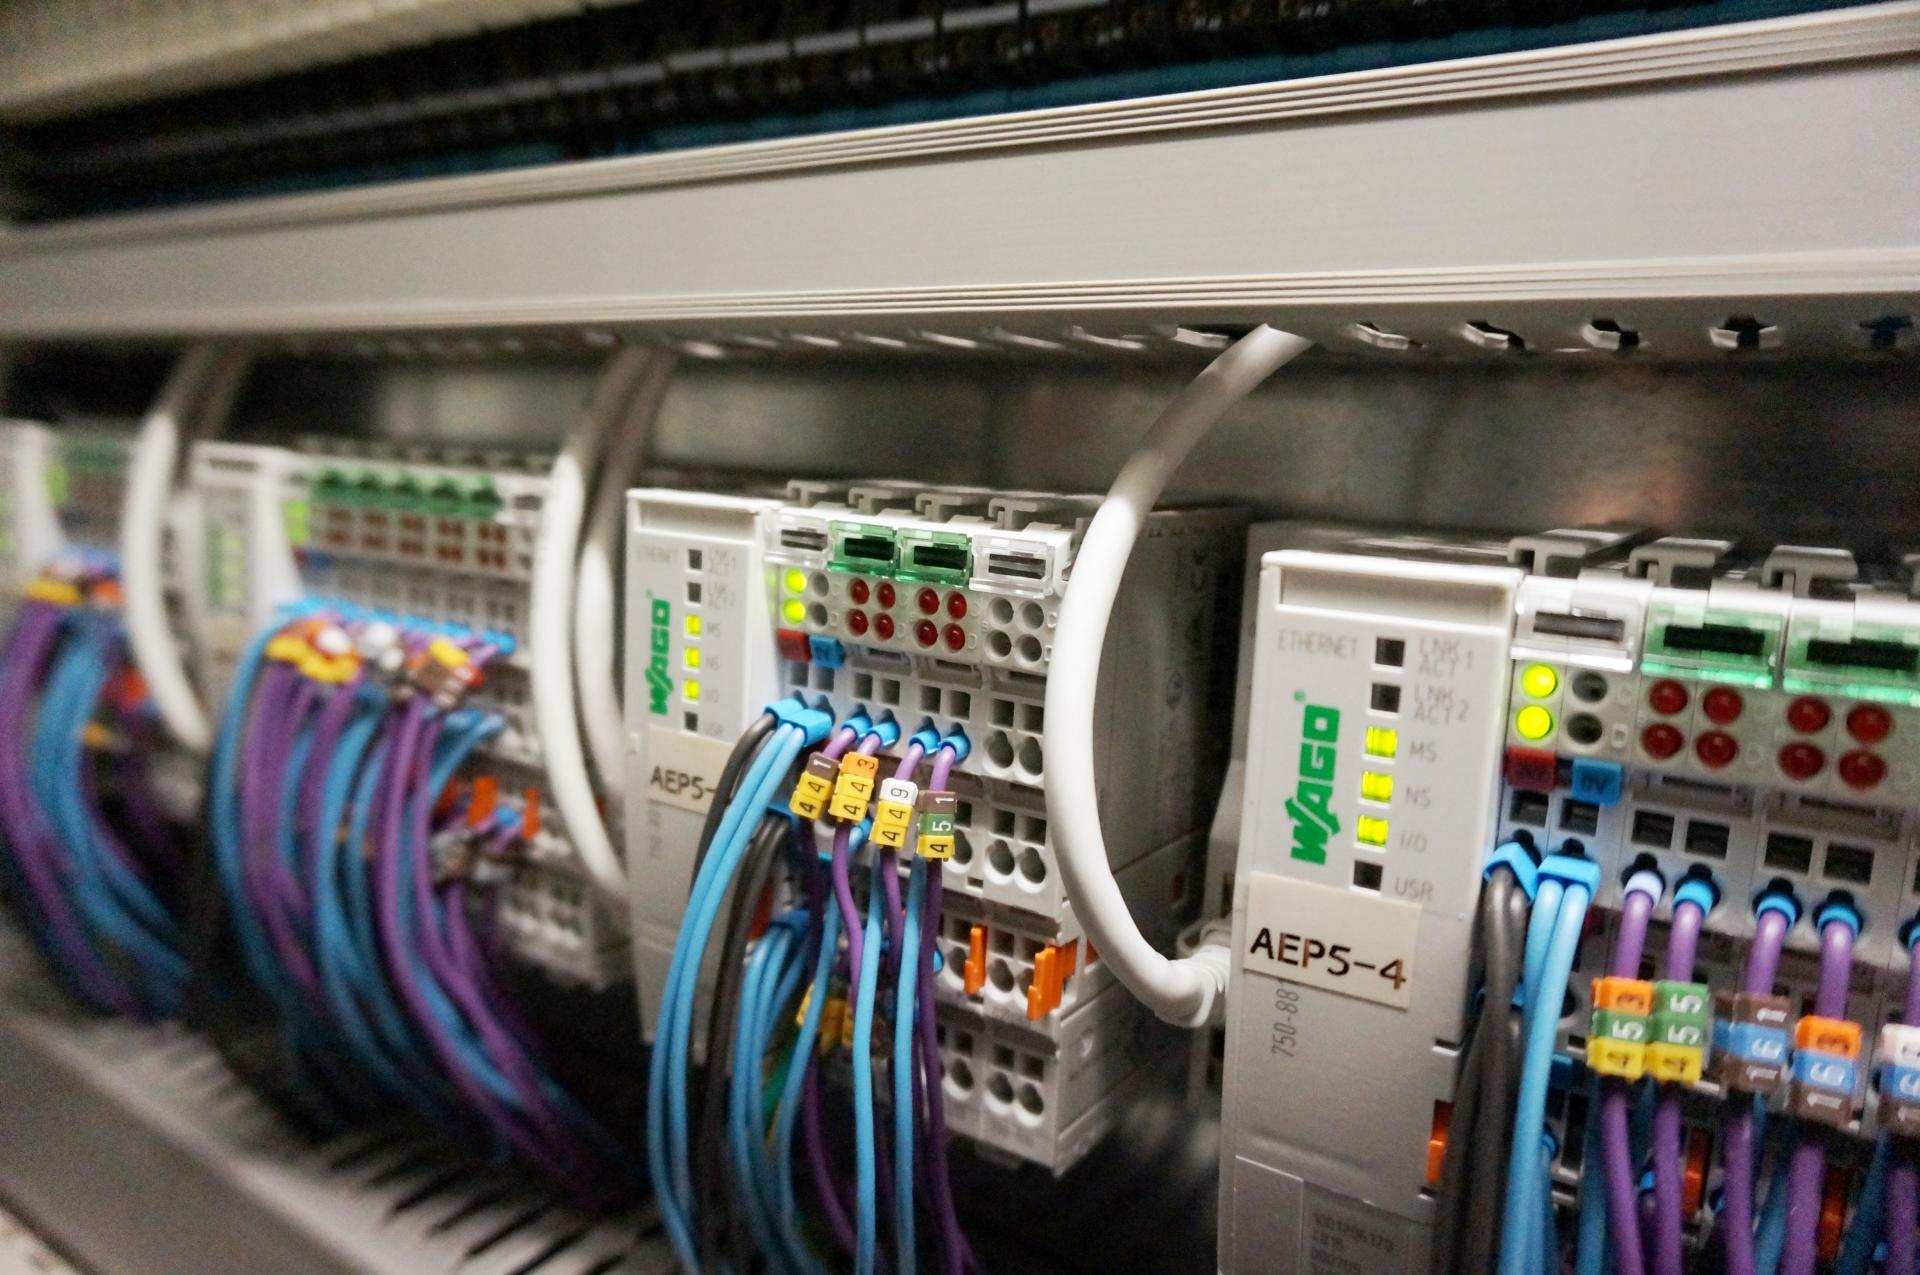
\includegraphics[width=0.7\textwidth]{data/plc.jpg}
\caption{Průmyslové \gls{plc} moduly. Převzato z~\texttt{wikimedia.org}.}
\label{fig:mtbusb-prototype}
\end{figure}

V~této práci se zaměříme na podmnožinu \gls{plc} modulů – totiž na takové,
jejichž hlavním úkolem je správně zpracovávat vstupní signály a~ovládat výstupní
periferie. Řízení logiky průmyslového procesu přenecháme počítači, s~kterým
\gls{plc} moduly komunikují.\footnote{V~praxi může \gls{plc} modul řídit logiku
procesu přímo, my však tuto situaci zkoumat nebudeme.}

Cílem této práce je navrhnout a implementovat novou verzi komunikační sběrnice
\gls{plc} obvodů \textit{\gls{mtbbus}} (\textit{Model Train
Bus}\footnote{Expanze zkratky do jejího plného významu nedává smysl, i~tak
budeme používat označení MTBbus, protože tak je zkratka zaužívaná.}).

\gls{mtbbus} je sběrnice, která se využívá pro řízení modelových kolejišť.
Je součástí systému \gls{mtb}. Skrze sběrnici lze číst signály z~kolejiště
(například polohy výhybek, obsazenost kolejových obvodů) a~povelovat prvky
v~kolejišti (návěstidla, přestavníky výhybek, přejezdy apod.). Obdobným
způsobem funguje zapezpečovací zařízení na skutečné železnici.

V~této práci autor nejprve popíše současné nasazení systému \gls{mtb}. Budou
formulovány důvody vedoucí k~nutnosti aktualizace sběrnice. Autor popíše, proč
jsou dostupná komerční řešení nevhodná a~navrhne vlastní nové (1) protokoly,
(2) hardwarové moduly a~(3) počítačové programy, které jím formulovaný problém
řeší.


\chapter{Současné nasazení sběrnice MTBbus} \label{chap:nasazeni}
Sběrnice \gls{mtbbus} vznikla okolo roku 2000, kdy se hledal vhodný systém pro
programovatelné počítačové řízení modelové železnice, spoluprací nadšenců
z~\textit{Klubu modelářů železnic Brno I} (dále jen \gls{kmz}) a \textit{Klubu
železničních modelářů Praha 3} \footnote{Je překvapivé, že
skupina nadšenců tehdy dokázala vytvořit systém, který by se mohl poměřovat se
současnými komerčními systémy řízení modelových kolejišť, viz dále.} \cite{mtb:web}.

\textit{Digital Command Control} (\gls{dcc}), dnes pravděpodobně
nejrozšířenější\footnotemark\\mezinárodně standardizovaný systém pro digitální
řízení modelové železnice \cite{dcc_intro:web} tehdy ještě nebyl v~České Republice
rozšířený. Navíc přirozeně vyvstal požadavek na minimalizaci nákladů
a maximalizaci nezávislosti na komerčních produktech jediného výrobce. Vznikl
tedy systém \gls{mtb}, který se pro řízení modelových kolejišť v \gls{kmz}
používá doteď \cite{kmz_rizeni:web}. Podotkněme, že systém \gls{mtb} se
do~dalších klubů po České Republice nerozšířil – nejspíš proto, že není
podporovaný komerčními softwary pro řízení modelové železnice a~že jej jeho
původní autor v~roce~2008 přestal podporovat.

\footnotetext{Autor této práce by rád odstranil slovo
\textit{pravděpodobně} a uvedl řádnou citaci. Bohužel neexistují studie, které
by bylo možné mohli citovat. Rozšířenost \gls{dcc} se zakládá na autorových
zkušenostech.}

\section{Popis sběrnice \gls{mtbbus}} \label{sec:mtbbus}

Každé kolejiště má svou vlastní sběrnici \gls{mtbbus}, ke které je připojený
právě jeden \textit{\gls{mtbusb} modul} a až \textit{255 \gls{mtb} modulů}.
\gls{mtbusb} modul řídí provoz sběrnice \gls{mtbbus} a~je připojen k~počítači.
\gls{mtb} moduly jsou pevně instalovány v~rámech kolejiště a~komunikují po
sběrnici \gls{mtbbus} s~\gls{mtbusb} modulem. Říkáme, že sběrnice je tzv.
\textit{single master, multiple slaves}. \gls{mtbusb} modul lze označit jako
\textit{master modul}, \gls{mtb} moduly jsou tzv. \textit{slave moduly}.
Celou situaci přehledně ilustruje obrázek \ref{fig:mtbbus-topology}.

Každý \gls{mtb} modul má:

\begin{compactenum}
\item 8bitovou adresu, která se konfiguruje \textit{jumpery} přímo na modulu,
\item konfiguraci (typ vstupů/výstupů, rychlost sběrnice, ...),
\item vstupy (stav vstupů),
\item výstupy (stav výstupů).
\end{compactenum}


\begin{figure}[ht]
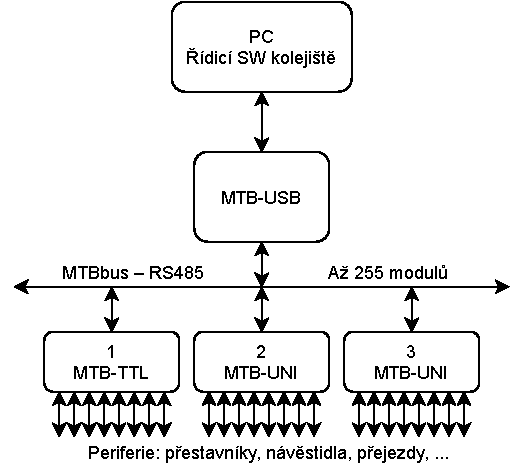
\includegraphics[width=0.7\textwidth]{data/mtb-topology.pdf}
\caption{Topologie systému \gls{mtb}.}
\label{fig:mtbbus-topology}
\end{figure}

\begin{table}[h]
	\begin{tabularx}{\textwidth}{XX}
		\toprule
		Typ přenosu & RS485, formát dat UART \\
		Komunikační rychlost & 38400~Bd, 57600~Bd, 115200~Bd \\
		Maximální počet modulů & 255 \\
		Počet datových bitů & 9 \\
		Stop bit & 1 \\
		Parita & žádná \\
		Maximální délka vedení & 100 m \\
		\bottomrule
	\end{tabularx}
	\caption{Základní parametry sběrnice \gls{mtbbus} \cite{mtbbus-specs}}
	\label{tab:mtbbus-params}
\end{table}

Současná sběrnice \gls{mtbbus} je založena na elektrickém standardu
\textit{RS485} \cite{mtbbus-specs}. Sběrnice RS485 je dvouvodičová (\textit{R+,
R-, GND}) vícebodová sériová poloduplexní komunikační průmyslová sběrnice
vyvinutá s~důrazem na odolnost vůči externímu rušení. Je vhodná pro přenos dat
na větší vzdálenosti, řádově až stovky metrů \cite{rs485-specs}. Pro dosažení
nejlepších elektrických vlastností by sběrnice měla být lineární. Sběrnice je
na obou koncích termínována rezistorem \textit{200 R} a~pull-up a~pull-down
rezistory pro držení definované úrovně signálu.

RS485 je velice snadno implementovatelná do prakticky všech mikrokontrolérů –
pro přístup ke sběrnici je třeba rozhraní UART, jeden pin pro řízení směru
komunikace a driver k~RS485.

\gls{mtb} moduly mohou být různého typu:

\begin{itemize}
\item \textbf{\gls{mtbuni}}

	\gls{mtbuni} (\textit{univerzální}) je nejpoužívanější typ modulu. Obsahuje
	16~digitálních vstupů a~16~digitálních výstupů. Na výstupech 0–7 umožňuje
	kódovat návěst protokolem S-COM\footnote{S-COM je jednoduchý jednosměrný
	komunikační protokol, který umožňuje přenášet návěsti návěstidel
	\cite{scom-specs}.}, což umožňuje připojení až 8 návěstidel k~jednomu
	\gls{mtbuni}. Modul dále umožňuje připojení IR čidel na
	vstupy\footnote{IR čidla jsou bodová čidla detekující průjezd vlaku, viz
	\ref{sec:ir}.}. Výstupy modulu jsou v~režimu otevřeného kolektoru
	s~maximální zátěží až 0.5~A~/~8~výstupů.

\item \textbf{MTB-TTL}

	\begin{figure}[ht]
	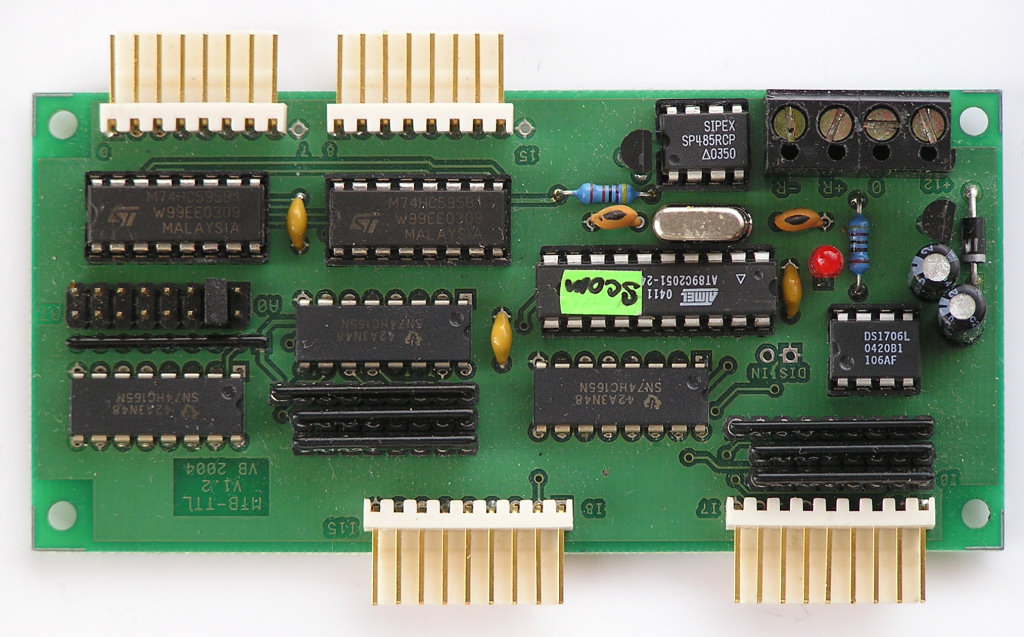
\includegraphics[width=0.7\textwidth]{data/mtbttl_foto.jpg}
	\caption{Ukázka modulu MTB-TTL \cite{mtb:web}.}
	\label{fig:mtbttl}
	\end{figure}

	MTB-TTL je zjednodušením modulu \gls{mtbuni}. Oproti \gls{mtbuni}
	nemá podporu IR čidel a~výstupy má v~režimu \gls{ttl}. Od tohoto typu
	modulu se v~současnosti ustupuje, neboť \gls{ttl} výstupy nejsou vhodné pro
	spínání vyšších napětí\footnote{např. pokud periferie na výstupu obashuje
	pull-up do +12~V} a~proto, že v~případě neaktivního výstupu (neaktivní =
	+5~V; inverzní logika) aktivně napájí výstupní port, což způsobuje nechtěné
	chování, například pokud je ne výstupním portu záměrně vypnutá periferie.
	V~krajním případě může dojít až k~přetížení TTL výstupu a jeho zničení. Na
	všechny nasazené moduly typu MTB-TTL byly postupně instalovány dodatečné
	obvody s~otevřenými kolektory na výstupy.

\item \textbf{MTB-REG}

	MTB-REG je modul umožňující generovat analogový výkonový výstup. Modul se
	připojí ke kolejím a řídí rychlost a~směr lokomotivy v~řízeném úseku kolejí.

	Tento způsob řízení jízdy (tzv. \textit{analogový}) je dnes již překonaný.
	V~současnosti se pro řízení jízdy lokomotiv na kolejišti používá tzv. systém
	\textit{Digital Command Control} (viz \ref{sec:dcc}), kde každá lokomotiva
	a mnohdy i~vagón v~sobě má mikroprocesor a~celý systém je řízen
	digitálně \cite{dcc_intro:web}.

	Modul MTB-REG je tedy již překonaným modulem a autor jej uvádí spíš pro
	úplnost popisu systému \gls{mtb}.

\item \textbf{MTB-POT}

	Modul MTB-POT obsahuje 4 analogové vstupy a 4 digitální vstupy. Jeho
	původním účelem bylo, aby se připojil k~potenciometru v~pultu obsluhy
	kolejiště, kterým obsluha reguluje jízdu vlaku. Po sběrnici přepošle data
	modulu MTB-REG a~tím dojde ke kýžené jízdě vlaku. Tento způsob řízení jízdy
	na kolejištích se již nepoužívá, proto i~modul MTB-POT na moderních
	kolejištích pozbývá svého smyslu.

\end{itemize}

Po sběrnici se komunikuje pevně definovaným protokolem.  Protokol definuje
příkazy pro moduly, odpovědi modulů, časování apod \cite{mtbbus-specs}.

Práce se sběrnicí z~pohledu aplikace v~počítači probíhá následovně:

\begin{compactenum}
\item Aplikace se připojí se k~MTB-USB modulu.
\item Aplikace provede sken aktivních modulů sběrnice.
\item Aplikace nahraje do všech aktivních modulů konfiguraci.
\item Aplikace přečte stav vstupů.
\item Aplikace zahájí provoz sběrnice – od této chvíle všechny moduly nahlašují
	změny stavů vstupů.
\item Aplikace čte vstupy, nastavuje výstupy a řídí provoz.
\item Aplikace ukončí provoz sběrnice a vynuluje stav výstupů \gls{mtb} modulů.
\item Aplikace uzavře spojení s~MTB-USB.
\end{compactenum}


\section{IR čidla} \label{sec:ir}

Nyní popíšeme princip fungování IR čidel v~kolejišti, protože bude v~dalších
kapitolách stěžejní.

IR čidlo je bodový detektor průjezdu vlaku. Do kolejí se vedle sebe umístí
opticky oddělená vysílací dioda a~fototranzistor, oba namířené vzhůru. Při
průjezdu vlaku dojde k~odrazu signálu od spodku vozu nebo lokomotivy, čímž je
detekován průjezd vlaku. Výhodou je nenápadná instalace mezi pražce, která
neruší celkový dojem modelu.

Pro spolehlivou detekci odrazu od matných černých povrchů podvozků je třeba
budit vysílací diodu vysokým proudem (až 200~mA), což vyžaduje použití
diody v~impulsním režimu. Současná \gls{mtbuni} deska podporuje IR čidla na
všech svých 16 vstupech, diody jsou buzeny tranzistory ve skupinách po
4~diodách.

\begin{figure}[ht]
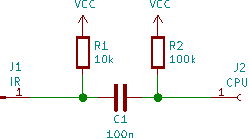
\includegraphics[width=0.5\textwidth]{data/cap-bind/capacitive-bind-example.pdf}
\caption{Zapojení vstupu kapacitní vazbou.}
\label{fig:cap-bind}
\end{figure}

Aby bylo zajištěno spolehlivé vyhodnocení odraženého signálu, je vstup
z~fototranzistoru zapojen na digitální vstup posuvného registru přes kapacitní
vazbu.

Vstupy \gls{mtbuni} desky se konfigurují osazením rezistorových lišt (běžný
vstup) nebo kondenzátorů (vstup z IR čidla). Kromě toho musí o~režimu pinu
vědět i~procesor, aby adekvátním způsobem zpracovával vstupní signál
\cite{mtbuni22-specs}.


\section{Systém \gls{mtb} v~kontextu řízení celého kolejiště} \label{sec:mtb_context}

V~\gls{kmz} je aktuálně systém \gls{mtb} nasazen na dvou kolejištích, další
nasazení je na modulovém kolejišti Mendelovy univerzity v~Brně, s~kterou klub
spolupracuje. Na těchto kolejištích je aktuálně nasazeno 99 \gls{mtb} desek.

Pro kontext uveďme, jak systém \gls{mtb} zapadá do celkové koncepce řízení
kolejiště. Viz schéma \ref{fig:control-topology}.

\begin{figure}[ht]
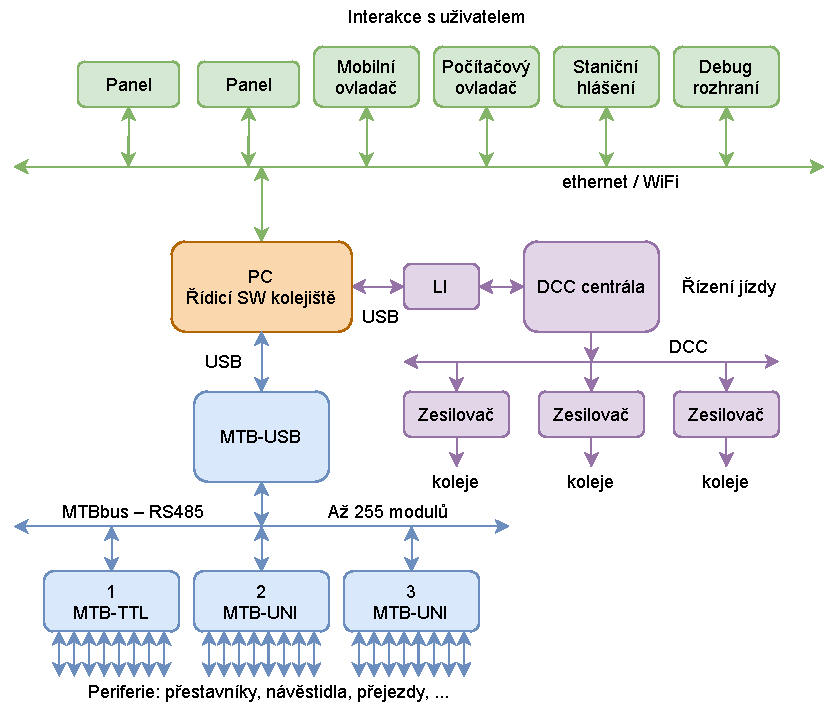
\includegraphics[width=\textwidth]{data/railroad-topology.pdf}
\caption{Schéma komponent řízení kolejiště v~\gls{kmz}.}
\label{fig:control-topology}
\end{figure}

Na první pohled je vidět, že kolejiště je řízeno dvěma různými systémy (modrá
a~fialová část diagramu).  Vyvstává otázka, proč je neintegrovat do systému
jednoho. Integrovaná řešení nabízejí majoritní výrobci hardwaru pro digitální
řízení modelové železnice.  Řízení jízdy i~trakce jedním systémem (\gls{dcc})
je rozšířeným přístupem jak v~Česku tak v~zahraničí. Všechna tato řešení jsou
však o~kompromisech, jak se dozvíme v~\ref{sec:dcc}. U~tvorby a~nasazení
systému \gls{mtb} stály osoby, které pracují na zabezpečení skutečné železnice.
Systém \gls{mtb} je tak oproti komerčně dostupným řešením řízení modelových
kolejišť navrhován s~důrazem na spolehlivost a~především bezpečnost.

Uveďme dva příklady za všechny: komerčně využívaná sběrnice RS pro snímání
stavu kolejiště nedokáže rozpoznat, že nějaký z~RS modulů (analogie \gls{mtb}
modulů) přestal fungovat \cite{rs:web}. Dále výstupní moduly nijak nepotvrzují,
že opravdu provedly akci, kterou počítač požaduje \cite{dcc_specs:web}. Tyto
příklady ilustrují, že komerčně dostupná řešení jsou podle autorova názoru blíže
hračce, než bezpečnému a~spolehlivému systému pro řízení modelů.

Poslední část schématu \ref{fig:control-topology} je část zelená, která
reprezentuje interakci s~uživatelem. \textit{Řídicí SW kolejiště} běží na
samostatném serveru, ke kterému se připojují všichni uživatelé systému –
dispečeři ze svých stanic, strojvedoucí ze svých ovladačů ale také třeba
technikové se svými diagnostickými nástroji nebo externí programy využívající
API serveru. Server kontroluje identitu uživatelů a umožňuje jim řídit ty
systémy, ke kterým mají uživatelé práva.

\section{Proč současný systém \gls{mtb} nedostačuje} \label{sec:mtb_fail}

Systém \gls{mtb} s~sebou nese řadu problémů.

\begin{enumerate}
\item \textbf{Licence, výrobní data}

U~současné implementace systému \gls{mtb} bohužel nebyly řádně vyřešeny licenční
podmínky mezi jeho autorem a~klubem. Souhrou událostí se \gls{kmz} dostal do
situace, kdy nemáme zdrojová data schémat a~layoutů desek plošných spojů ani
zdrojové kódy firmwarů.

Aktuální situace tak prakticky znemožňuje výrobu dalších \gls{mtb} desek,
o~záměru chtít systém \gls{mtb} nabízet mimo klub ani nemůže být řeč.

\item \textbf{Hardware}

Systém \gls{mtb} zaznamenal poslední aktualizaci hardwarových komponent v~roce
2007. V~současné době jsou některé použité součástky bohužel prakticky
nesehnatelné, což znemožňuje výstavbu dalších částí kolejiště. To je zcela
zásadní problém.

\item \textbf{Software}

Současné MTB moduly využívají procesory \textit{AT89C2051} (2~kB FLASH,
128~B SRAM). Tyto procesory svými parametry odpovídají době návrhu celého
systému. Firmware v~procesorech naráží na jejich hardwarové limity – do
procesoru se jednoduše nevejde další logika, což efektivně zabraňuje přidání
nových funkcí. Procesorům navíc chybí některé klíčové periferie, například
EEPROM paměť.

\end{enumerate}

Současný systém \gls{mtb} byl vyhodnocen jako celkově nedostatečný, je potřeba
ho buď aktualizovat nebo nahradit za systém jiný.

Na náhradu systému \gls{mtb} autor práce stanovil především následující
požadavky.

\begin{compactenum}
\item Systém musí být kompatibilní se současným řídicím softwarem kolejiště.
\item Systém musí být kompatibilní se současným hardwarem kolejiště.
\item Systém musí být udržitelný minimálně 20~let.
\item Finanční náklady a~čas vložený do povýšení současného systému na nový
	systém by měly být minimalizovány.
\item Systém musí být schopen potvrzovat akce řídicího počítače a~evidovat správnou
	funkčnost modulů.
\item Systém by měl být rozšiřitelný co se týče podporované funkcionality –
	nové požadavky na funkcionalitu by mělo být možné implementovat.
\end{compactenum}

K~naplnění těchto požadavků lze přistoupit dvěma různými způsoby: zakoupením
komerčního produktu nebo vytvořením produktu vlastního. Prozkoumejme nejprve,
jestli existují komerční řešení, která naplňují definované požadavky.


\chapter{Existující řešení} \label{chap:existujici-reseni}
Nyní představíme v~současnosti nejrozšířenější systémy pro \textit{digitální}
řízení modelové železnice. Prozkoumáme zařízení, která tyto standardy
podporují, a~zhodnotíme jejich vlastnosti. Bude vyhodnoceno, jestli zařízení
naplňují požadavky definované v~předchozí kapitole.

\section{Digital Command Control} \label{sec:dcc}

\textit{Digital Command control} (\gls{dcc}) je celosvětově nejrozšířenější
systém pro \textit{digitální}\footnote{\textit{Digitální} znamená, že mezi
jednotlivými prvky řízení proudí digitální data.} řízení modelové železnice
\cite{dcc_systems:web}. K~\gls{dcc} existují alternativy, které však v~Evropě
nejsou rozšířené, proto alternativní systémy nebudeme uvažovat.\footnote{Toto
tvrzení se zakládá na autorových zkušenostech, relevantní studie neexistují.}

\gls{dcc} specifikuje, které komponenty se účastní řízení kolejiště a jak se
tyto komponenty mají chovat – od elektrických standardů (např. doporučený
způsob zapojení vodičů pod kolejištěm) až po komunikační protokoly. \gls{dcc}
je otevřený standard vytvořený organizací \textit{National Model Railroad
Association} (\gls{nmra}), která sdružuje modelářské kluby (a~tedy i~modeláře),
které jsou přímými uživateli systému \gls{dcc}. Systém \gls{dcc} je tedy
navržen modeláři k~naplnění potřeb modelářů.

Jednotlivé prvky systému \gls{dcc} jsou znázorněny v~\ref{fig:dcc-overview}.
Nyní tyto prvky stručně popíšeme.

\begin{figure}[ht!]
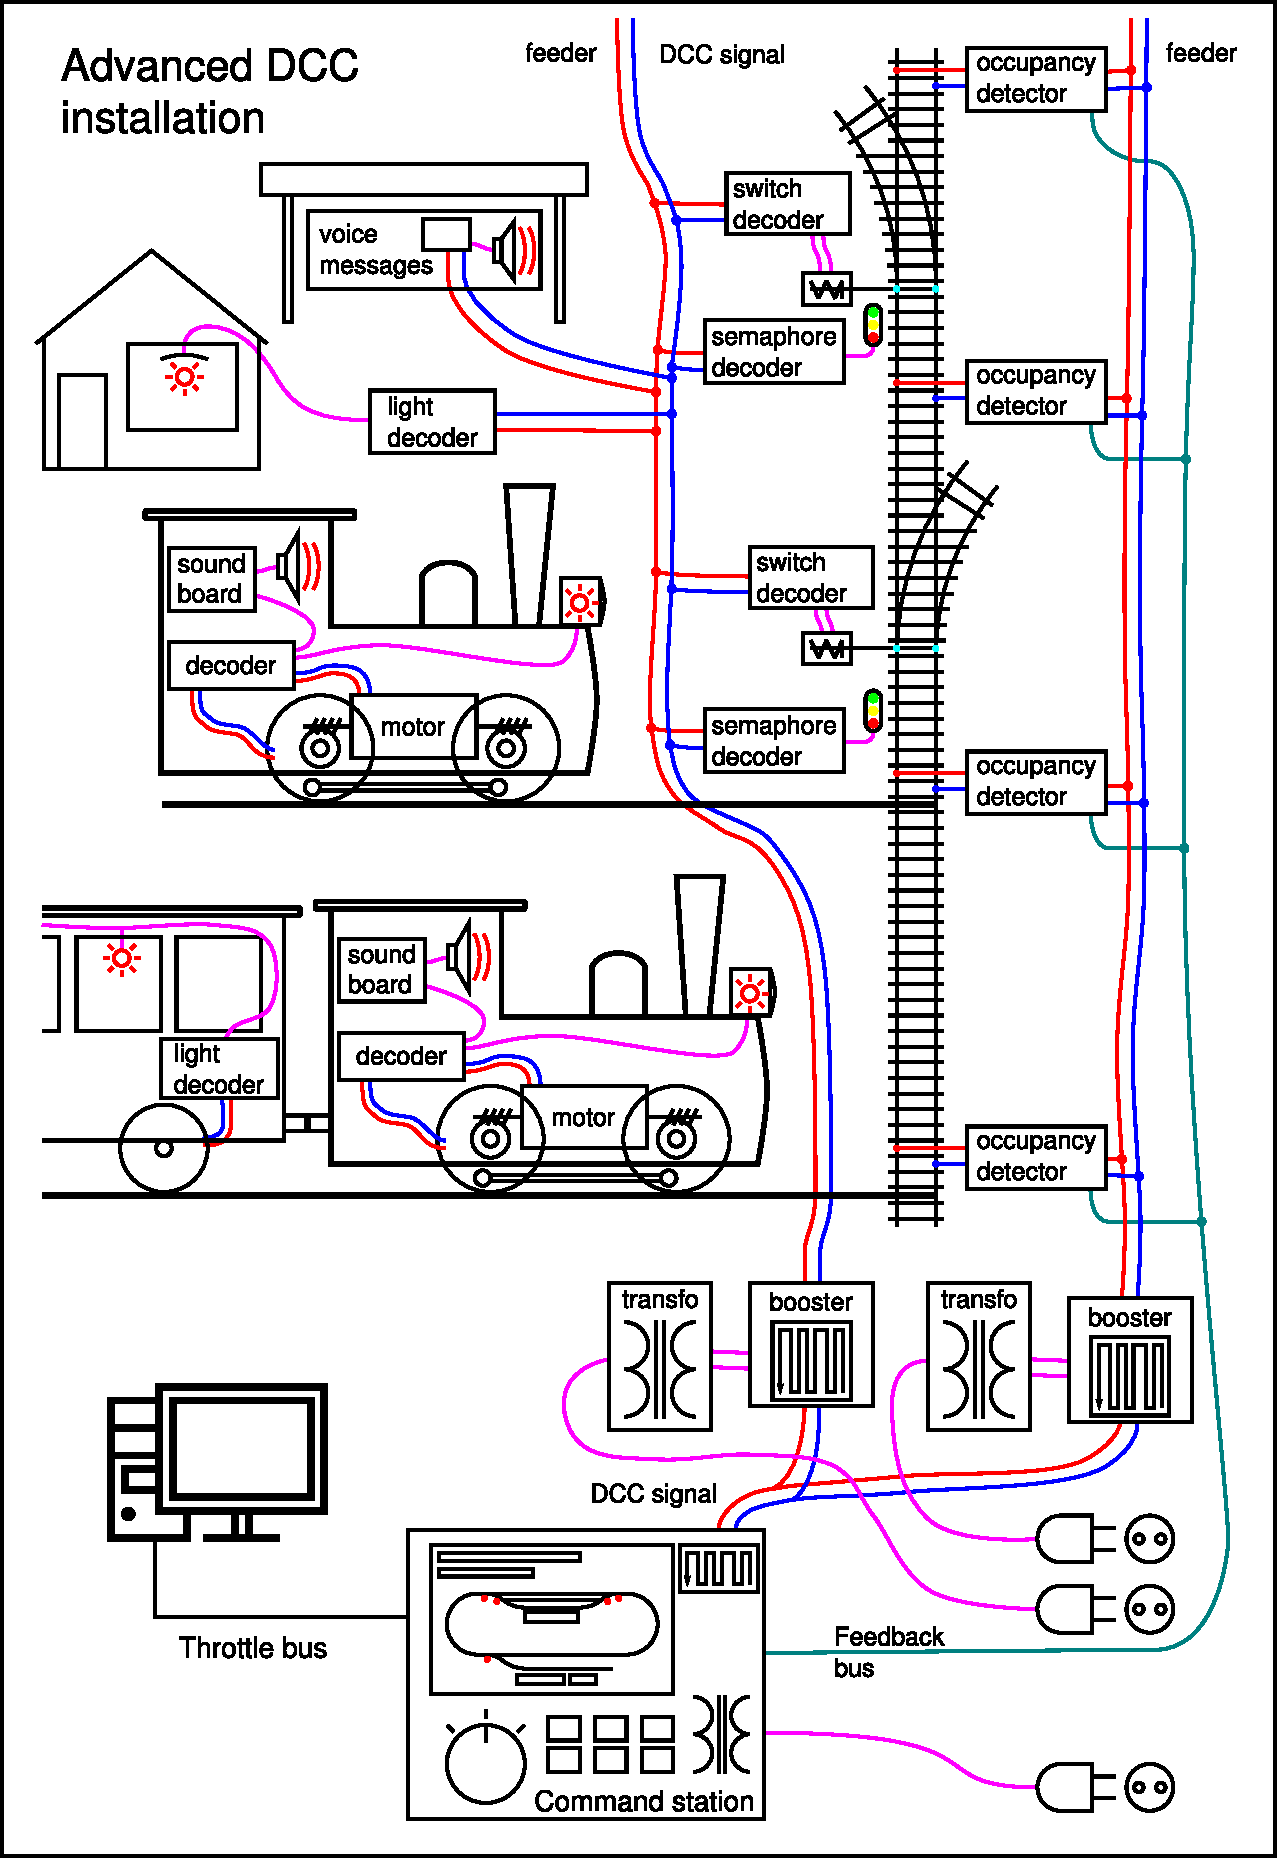
\includegraphics[width=0.95\textwidth]{data/schema_dcc_en.pdf}
\caption{Schéma systému \gls{dcc}. Převzato a upraveno z~\cite{dcc_wikipedia:web}.}
\label{fig:dcc-overview}
\end{figure}

Základní komponentou celého systému je \textit{DCC centrála (Command Station)},
která má 3 hlavní úkoly.

\begin{compactenum}
\item Číst stav \textit{modulů zpětného hlášení} přes \textit{sběrnici zpětného hlášení \\
	(feedback bus)}.
\item Povelovat \textit{dekodéry} (lokomotiv, přestavníků, návěstidel apod.).
\item Obousměrně komunikovat po \textit{sběrnici ovladačů (throttle bus)}.
\end{compactenum}

Řízení dekodérů centrála provádí generováním \textit{DCC signálu} (červený
a~bílý vodič ve schématu \ref{fig:dcc-overview}), do kterého centrála kóduje
operace požadované po dekodérech – např. \uv{dekodére číslo 541, zastav
lokomotivu}, \uv{dekodére číslo 4741, aktivuj čelní světla}.

Ke sběrnici ovladačů jsou připojené buď fyzické ovladače, nebo počítače.
Operátor provozu zadává příkazy, například otočením kolečka ovladače nebo
interakcí s~příslušným software, tyto příkazy jsou přeposlány do centrály,
centrála je dále přeposílá dekodérům, které přímo vykonávají požadované akce.

Na \textit{sběrnici zpětného hlášení} jsou připojeny moduly s~digitálními vstupy,
které jsou namontovány pevně v~kolejišti a~které čtou stav periferií.
Centrála informuje uživatele skrze \textit{sběrnici ovladačů} o~změnách ve
stavech vstupů \textit{modulů zpětného hlášení}. Vstupy modulů zpětného hlášení
jsou připojené například k~signalizacím obsazení \textit{kolejových obvodů},
takže uživatel nebo řídicí SW pozná, že se na koleji nachází nebo nenachází
vlak, dále například koncovým spínačům poloh výhybek, takže řídicí software je
schopen zabezpečit \textit{vlakovou cestu}.

Pro úplnost uvedeme všechny typy vstupů a~výstupů, které se v~\gls{kmz}
používají.

Výstupy:

\begin{compactitem}
\item řízení jízdy lokomotiv,
\item řízení osvětlení lokomotiv a vozů,
\item řízení zvuků lokomotiv,
\item nastavení polohy výhybky, výkolejky,
\item rozpojovač,
\item návěstidlo,
\item přejezd,
\item statické pouliční nebo domovní osvětlení,
\item indikace v~pultu obsluhy.
\end{compactitem}

Vstupy:

\begin{compactitem}
\item indikace obsazení kolejového obvodu,
\item indikace bodového průjezdu vlaku daným místem skrze infračervené čidlo
	(viz \ref{sec:ir}),
\item indikace koncové polohy výhybky,
\item indikace stavu přejezdu,
\item tlačítka v~pultu obsluhy.
\end{compactitem}

Všimněme si klíčové vlastnosti systému: pro řízení dekodérů
a~pro sběr informací z~kolejiště jsou použity 2~různé sběrnice: \textit{dcc
signál} a~\textit{sběrnice zpětného hlášení}. Platí totiž, že signál \gls{dcc}
je pouze jednosměrný. Signál putuje z~\gls{dcc} centrály přes
\textit{zesilovače} a přes koleje do lokomotiv a~vozů, které poveluje.
Existují jen velice omezené prostředky jak dostat data z~lokomotivy zpět do
\gls{dcc} centrály\footnote{Takovému systému říkáme \textit{RailCom}
\cite{railcom:web}.}. Tyto prostředky navíc vznikly až v~pozdějších verzích
normy \gls{dcc}, takže dnes nejsou všeobecně zaužívané \cite{railcom:web}.
Sběrnice \gls{dcc} je tedy prakticky vzato jednosměrná, dokonce bez odpovědí
dekodérů na příkazy

To znamená, že centrála musí DCC příkazy posílat opakovaně, aby zaručila, že je
dekodér skutečně přijme. Může se totiž snadno stát, že lokomotiva zrovna není
schopna přijímat signál – například jede po špinavých kolejích, ze kterých
špatně sbírá. Problém s~přijímáním dat vlivem špatného kontaktu se netýká
\textit{dekodérů příslušenství} (na obrázku \ref{fig:dcc-overview}
\textit{switch decoder} a \textit{semaphore decoder}).  Tyto dekodéry jsou
připojeny pevným kabelem ke kolejím, takže mají nejlepší předpoklady dekódovat
\gls{dcc} signál korektně. Stále však platí, že dekodér neodpoví, že přijal
a~provedl povel. Vykonání povelu mohlo být narušeno čímkoliv od
elektromagnetického rušení signálu až po nepřijetí povelu vlivem chyby ve
firmwaru dekodéru.

Může se zdát, že samotný protokol \gls{dcc} nesplňuje požadavky popsané
v~\ref{subsec:gen_requirements} a~proto jej nemá smysl uvažovat jako nástupce
současného systému \gls{mtb}. Ačkoliv striktně vzato je tento závěr
správný, je nutné si uvědomit širší souvislosti.

Pří řízení provozu na modelovém kolejišti sledujeme mnohé cíle, z~nichž na
prvním místě stojí bezpečnost. Na skutečné železnici je bezpečnost samozřejmě
mnohem důležitější než na železnici modelové. Přesto například materiální škody
vzniklé projetím návěsti zakazující jízdu, vykolejením soupravy, srážky nebo
následného pádu modelu na zem jsou tak markantní, že bezpečnost provozu je
třeba řešit.

Bezpečnost řízení provozu železnice skutečné i~modelové stojí na tom, že
nepustíme vlak do míst, kde by mu hrozila nehoda. K~nehodě může dojít dvěma
způsoby.

\begin{enumerate}
\item \textbf{Vlak stojí a~je nesprávně rozjet do místa, které pro něj není
bezpečné.}

	I~přes to, že dekodéry nepotvrzují přijetí signálu a~provedení akce, této
	situace se jsme schopni vyvarovat. Všechny klíčové komponenty kolejiště,
	které řídí směr pohybu vlaku (výhybky, výkolejky) indikují svůj stav. To
	znamená, že když se nepovede provést například přestavení výhybky vlivem
	nedoručení příslušného \textit{\gls{dcc} paketu}, výhybka se nepřestaví,
	moduly zpětného hlášení správně indikují, že výhybka se nehýbe, řídicí
	software správně vyhodnotí, že nedošlo ke splnění podmínek pro rozjetí
	vlaku a~vlak nerozjede.

	Z~tohoto pohledu tedy nepotvrzování \gls{dcc} příkazů nevede k~nebezpečné
	situaci.

	Jiná situace nastane u~dekodérů, které provádějí akce, aniž by indikovaly
	svůj stav. Takové dekodéry jsou například \textit{dekodéry návěstidel}
	(\textit{semaphore decoder} na obrázku \ref{fig:dcc-overview}). Tyto dekodéry
	však neovlivňují směr jízdy vlaku. Špatná návěst na návěstidle je
	nemodelová, ale ke hmotným ztrátám nedojde.
	\footnote{Jiná situace panuje na skutečné železnici, kde je návěst návěstidla
	důležitým komunikačním prvkem mezi dispečerem a~strojvedoucím. Je nutné,
	aby strojvedoucí viděl správnou návěst, protože nesprávná návěst
	by mu mohla povolit jízdu, přestože se například proti němu blíží vlak. Nebo
	by například mohla povolit jízdu vyšší rychlostí, než jaká je v~daném
	úseku předepsaná a~vlak by pak nemusel stihnout později zabrzdit. Proto se
	na skutečné železnici kontroluje, že světly návěstidel, která mají být
	rozsvícená, skutečně prochází proud.}

\item \textbf{Vlak se nepovede zastavit.}

	Může nastat situace, kdy se vlak blíží k~místu zastavení, řídicí software
	mu správně pošle příkaz k~zastavení, ale lokomotiva přesto nezastaví.
	Například vlivem již popsaného špatného kontaktu lokomotivy s~kolejemi
	a~tudíž neschopnosti řádně dekódovat \gls{dcc} signál. Norma \gls{dcc} totiž
	specifikuje \uv{pokud dekodér nedekóduje signál, zůstává ve stejném stavu}.
	Tedy například lokomotiva se pořád pohybuje vpřed.

	Popsaná situace v~praxi nastává, ale není v~záběru této práce s~ní naložit.
	Tato práce se zaměřuje především na řízení příslušenství a~snímání stavu
	kolejiště, nikoliv na systém řízení jízdy hnacích vozidel.

\end{enumerate}

Závěrem uveďme, že z~dosavadního popisu systému \gls{dcc} plyne, že tento
systém je pro řízení příslušenství vhodný, i~když s~drobnými nedokonalostmi.

\subsection{Sběrnice zpětného hlášení}

V~předchozí kapitole jsme při formulování závěrů vycházeli z~předpokladu, že
jsme schopni bezpečně indikovat stav všech prvků v~kolejišti (pomocí
\textit{sběrnice zpětného hlášení} – \textit{feedback bus} ve schématu
\ref{fig:dcc-overview}). Prozkoumejme spolehlivost této sběrnice.

\gls{nmra} nedefinuje jednotný standard pro \textit{sběrnici zpětného hlášení}
\cite{dcc_specs:web}, různí výrobci používají různé (vlastní) sběrnice
\cite{dcc_feedbacks:web}. Analyzujme nejpoužívanější sběrnice.

\subsubsection{S88}

\textit{S88} je základní sběrnice zpětného hlášení. Její fungování lze v~zásadě
charakterizovat jako \uv{vylepšené posuvné registry} \cite{s88:web}. Jednotlivé
moduly jsou řazeny za sebe, propojují se vždy sousední moduly. První modul je
připojen do \gls{dcc} centrály.

\begin{figure}[ht!]
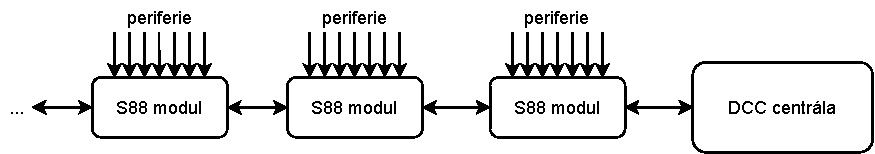
\includegraphics[width=\textwidth]{data/s88.pdf}
\caption{Topologie sběrnice S88.}
\label{fig:s88-topology}
\end{figure}

\textit{S88} je nízkonákladová sběrnice určená pro malá kolejiště. Limitujícím
faktorem je především napájení z~5~V, které není vhodné na delší rozvody,
a~malá odolnost proti rušení \cite{s88:web}.

Jak je patrné z~topologie sběrnice \ref{fig:s88-topology}, při výpadku
(napájení) jednoho modulu jsou ztracena data i~ze všech dalších modulů dále od
centrály. Takové chování je pro profesionální \gls{plc} systém nevhodné.

\subsubsection{RSbus}

\textit{RSbus} je sběrnice firmy \textit{Lenz Elektronik}. Oproti \textit{S88}
je organizována do topologie sběrnice. Jednotlivé moduly jsou napájeny
samostatně, sběrnice je dimenzovaná až na 128 modulů, každý s~8 digitálními
vstupy \cite{rs:web} \cite{rs_lib:web}.

\begin{figure}[ht!]
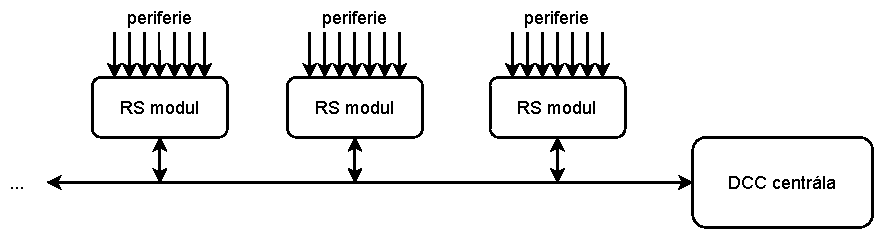
\includegraphics[width=\textwidth]{data/rs.pdf}
\caption{Topologic sběrnice RSbus.}
\label{fig:rs-topology}
\end{figure}

Komunikaci po sběrnici řídí \gls{dcc} centrála – posílá výzvy jednotlivým
modulům a~moduly odpovídají, pokud mají nějaká data k~odeslání. Moduly odesílají
data jen pokud došlo ke změně vstupů, což znamená, že nelze odlišit nefunkční
modul od funkčního modulu se setrvalým stavem vstupů \cite{rs_lib:web}.

Takové chování bohužel nesplňuje požadavky definované
v~\ref{subsec:gen_requirements}. Pokud by například došlo výpadku \textit{RS
modulu} a~následnému obsazení kolejového obvodu, jehož stav tento modul indikuje,
z~pohledu řídicího softwaru by byl kolejový obvod stále volný. Řídicí software
by pak povolil vjezd vlaku na obsazenou kolej, čímž by způsobil srážku.

K~výpadku RS modulu může dojít snadno například ztrátou napájení vlivem chybné
obsluhy, reakce pojistky na přetížení, poruchy apod.

\subsubsection{LocoNET}

Poslední z~analyzovaných sběrnic je \textit{LocoNET}. LocoNET je
proprietární sběrnice společnosti \textit{Digitrax} \cite{loconet:web}, jejíž
plná specifikace není volně dostupná \cite{loconet_license:web}.  Plné použití
této sběrnice podléhá licenčním poplatkům \cite{loconet_license:web}.
Zajímavou vlastností sběrnice je, že slučuje sběrnice \textit{throttle bus}
a~\textit{feedback bus} (viz schéma \ref{fig:dcc-overview}). Řídicí software
v~počítači tak může přímo dotazovat moduly zpětného hlášení a~úplně tak obejít
\gls{dcc} centrálu. Sběrnice LocoNET je navíc obousměrná,
LocoNET moduly jsou vstupně-výstupní, takže počítač může přímo
povelovat periferie \cite{loconet:web}. Viz \ref{fig:loconet-topology}.

\begin{figure}[ht!]
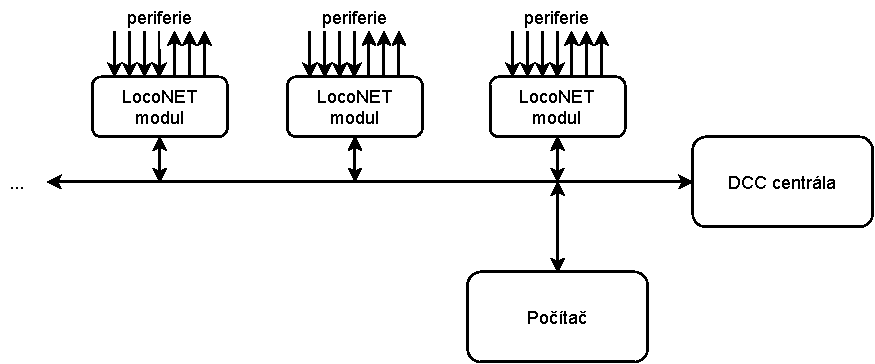
\includegraphics[width=\textwidth]{data/loconet.pdf}
\caption{Topologic sběrnice LocoNET.}
\label{fig:loconet-topology}
\end{figure}

Sběrnice LocoNET umožňuje počítači zjišťovat stav modulů přímou komunikací bez
zapojení centrály \cite{loconet-specs}, takže počítač může rozpoznat, které
moduly jsou na sběrnici přítomny, výpadek modulu a~oživení modulu po výpadku.

Sběrnice LocoNET splňuje požadavky na bezpečné řízení periferií
definované v~\ref{subsec:gen_requirements}. Při bližší inspekci však
zjišťujeme, že nasazení této sběrnice by znamenalo nakoupit a~vyměnit cca 100
modulů v~kolejišti. Výměna by navíc musela být rozsáhlejší, LocoNET
moduly přímo nepodporují například generování signálu \textit{\gls{scom}}. Pro
nasazení sběrnice LocoNET by musely být instalovány přídavné moduly
pro řízení návěstidel.

\section{BiDiB}

Zajímavou alternativou k~systému \gls{dcc} je sběrnice \textit{\gls{bidib}}
\footnote{\url{http://bidib.org/}} (\textit{BiDirectional Bus}). \gls{bidib}
je komunitní sběrnice s~otevřeným protokolem, která do velké míry splňuje
všechny požadavky definované v~\ref{subsec:gen_requirements}. Systém \gls{bidib}
lze provozovat na více komunikačních médiích (RS485, Ethernet, sériový port),
návrh systému je podobný návrhu \gls{usb} – na sběrnici je jeden \textit{master},
až 32 \textit{slave} v~každém segmentu, přičemž jedním ze \textit{slave} může
být \textit{hub} vedoucí do dalšího segmentu.

Autoři \gls{bidib} si dali za cíl, podobně jako autor této práce, vytvořit
bezpečný systém pro řízení modelových kolejišť. Systém tak podporuje potvrzování
příkazů, aktualizaci firmwaru modulů apod.

Pro nasazení \gls{bidib} by bylo třeba provést netriviální úpravy
aktuálních modulů kolejiště – \gls{bidib} například definuje standardní
konektory pro propojení modulů. Dále by bylo třeba vyřešit, jak naložit
s~limitem 32 desek v~jednom segmentu sběrnice (protože \gls{mtbbus} je navržen
až pro 255 modulů) a~s~jiným způsobem adresování modulů sběrnice.
\section{Závěr}

V~této kapitole byly popsány základní přístupy k~řízení moderní digitální
modelové železnice. Bylo zkoumáno, jestli komerční produkty splní požadavky
definované v~\ref{subsec:gen_requirements}. Po vyloučení technicky
nezpůsobilých řešení zbyly sběrnice LocoNET (s~poznámkou,
že její nasazení by bylo finančně náročné a~pracné) a \textit{\gls{bidib}}.

Při uvažování sběrnice LocoNET vyvstal problém s~integrací ovládání
návěstidel. Tento problém je obecnějšího rázu – jakékoliv komerční řešení není
schopné nabídnout takovou flexibilitu, jakou bychom v~\gls{kmz} potřebovali.
Je nutné integrovat systém řízení kolejiště se současnými periferiemi, ale
i~s~periferiemi budoucími. Je chtěné mít možnost pružně reagovat na nové
periferie, které se objeví například za 10 let.

Uvažme také aspekt zpětné kompatibility – vlastní systém nám umožní co možná
nejrozumněji zachovat kompatibilitu se stávajícím systémem řízení kolejiště
a~minimalizovat tak finanční náklady a čas nutný pro aktualizaci systému.
Nutnost rozumné zpětné kompatibility tak fakticky vylučuje i~nasazení
\gls{bidib}.

Vnímejme tuto kapitolu tedy především jako přehled technologií, které se
při řízení současné digitální modelové železnice používají. Přistupme k~návrhu,
jak povýšit systém \gls{mtb} výrobou vlastních komponent.


\chapter{Závěr} \label{chap:zaver}
Tato diplomová práce demonstrovala, že pro vytvoření plnohodnotného \gls{plc}
systému je třeba zvládnout širokou škálu dílčích kroků. Od návrhu komunikačních
protokolů, přes návrh hardwaru, programování firmwaru, až po programování
počítačových aplikací a~knihoven. Autorovi se povedlo všechny tyto kroky
úspěšně provést. Podařilo se mu vytvořit

\begin{compactitem}
\item nový protokol \gls{mtbbus},
\item nový master modul sběrnice \gls{mtbbus} (\gls{mtbusb} v4),
\item nový univerzální \textit{slave} modul sběrnice \gls{mtbbus} (\gls{mtbuni} v4),
\item nástavný modul do starších modulů \gls{mtbuni} (MTB-2-AVR),
\item počítačovou aplikaci pro přístup k~systému \gls{mtb} (MTB Daemon),
\item knihovnu pro integraci nového \gls{mtb} do současného řídicího systému
	kolejiště (hJOP MTB Network RCS Library)
\end{compactitem}

Komponenty vytvořené v~rámci této práce a~jejich interakce jsou přehledně
zobrazeny v~\ref{fig:new-topology}.

\begin{figure}[ht]
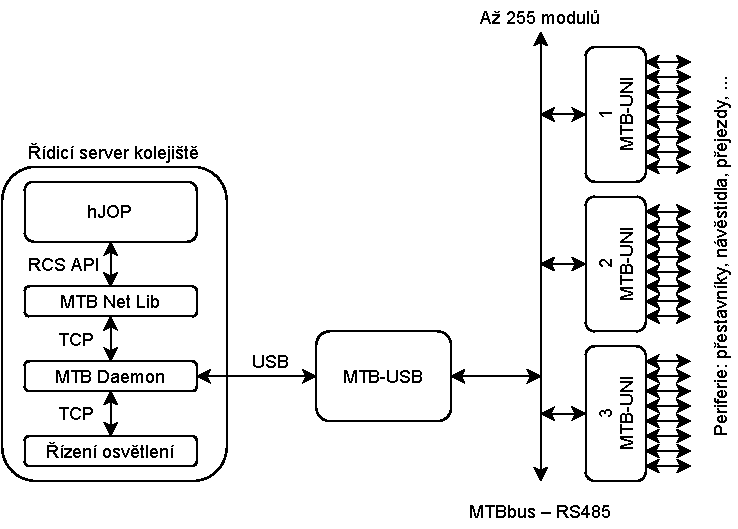
\includegraphics[width=0.8\textwidth]{data/new-topology.pdf}
\caption{Komponenty vytvořené v~rámci diplomové práce (mimo \textit{hJOP}
a~\textit{Řízení osvětlení}).}
\label{fig:new-topology}
\end{figure}

V~rámci práce byly formulovány požadavky (\ref{sub:mtbbus-req-summary}), které
má nový systém \gls{mtb} splnit. Všechny tyto požadavky byly naplněny.
Podařilo se vytvořit systém, který za poměrně malé finanční a časové náklady
značně povyšuje současný systém \gls{mtb}. Především však vznikl otevřený
a rozšiřitelný systém s~výhledem udržitelnosti po desítky let. Nový systém
\gls{mtb} umožní stavbu dalších kolejišť, udržování a rozšiřování kolejišť
současných. Nový systém \gls{mtb} si může vyrobit každý, kdo bude chtít bezpečně
řídit své modelové kolejiště.

Pro \gls{kmz} znamená \gls{mtb} v4 možnost nasadit více řídicích systémů
kolejiště, a~konečně tak zprovoznit řízení osvětlení, řízení tramvajové
a~autobusové dopravy. \gls{mtb} v4 umožní nasazení pultů obsluhy,
vytvoření nových chytrých zesilovačů \gls{dcc} signálu. Umožní výstavbu nového
depa kolejových vozidel, kde se budou používat speciální \gls{mtb} moduly.
Pro \gls{kmz} je \gls{mtb} v4 velkým krokem vpřed.

\gls{mtb} v4 bylo nasazeno na testovacím kolejišti o~20 modulech, kde úspešně
funguje.

\section{Možná rozšíření} \label{sec:future}

Při návrhu tak velkého systému, jako je \gls{mtb}, se přirozeně ukázaly mnohé
cesty, které by bylo možné v~budoucnu prozkoumat.

Systém \gls{mtb} by v~budoucnu mohl podporovat vyšší rychlosti komunikace nebo
automatickou detekci rychlosti sběrnice. \gls{mtb} by mohlo být rozšířeno
o~jednotky, které provádějí retranslaci dat sběrnice bezdrátově (pro vzdálené
připojení modulů).

Jednou z~otázek týkajících se budoucího rozšíření je, jak umožnit, aby systém
\gls{mtb} mohl interagovat s~komerčními softwary pro řízení modelových
kolejišť.
Dalším možným rozšířením je tak implementovat do majoritních komerčních
softwarů pro řízení modelových kolejišť podporu pro \gls{mtb}. Některé softwary
jsou však uzavřené. Pro takové softwary by bylo možné napsat alternativní
firmware do \gls{mtbusb}, který by zajistil, že \gls{mtbusb} modul se pro
počítač bude tvářit jako některý z~komerčních systémů pro řízení kolejišť.

Dalším přirozeným způsobem rozšíření, který má autor této práce v~plánu
v~nejbližším roce uskutečnit, je přidání dalších typů modulů. V~budoucnu
vzniknou \gls{mtb} moduly pro chytré zesilovače \gls{dcc} signálu,
\textit{RailCom} detektory a jiné. Systém \gls{mtb} je na tato rozšíření
připraven.


\printbibliography[heading=bibintoc]

\appendix
\chapter{Přílohy} \label{chap:appendix}
\vspace{-2em}

\begin{figure}[H]
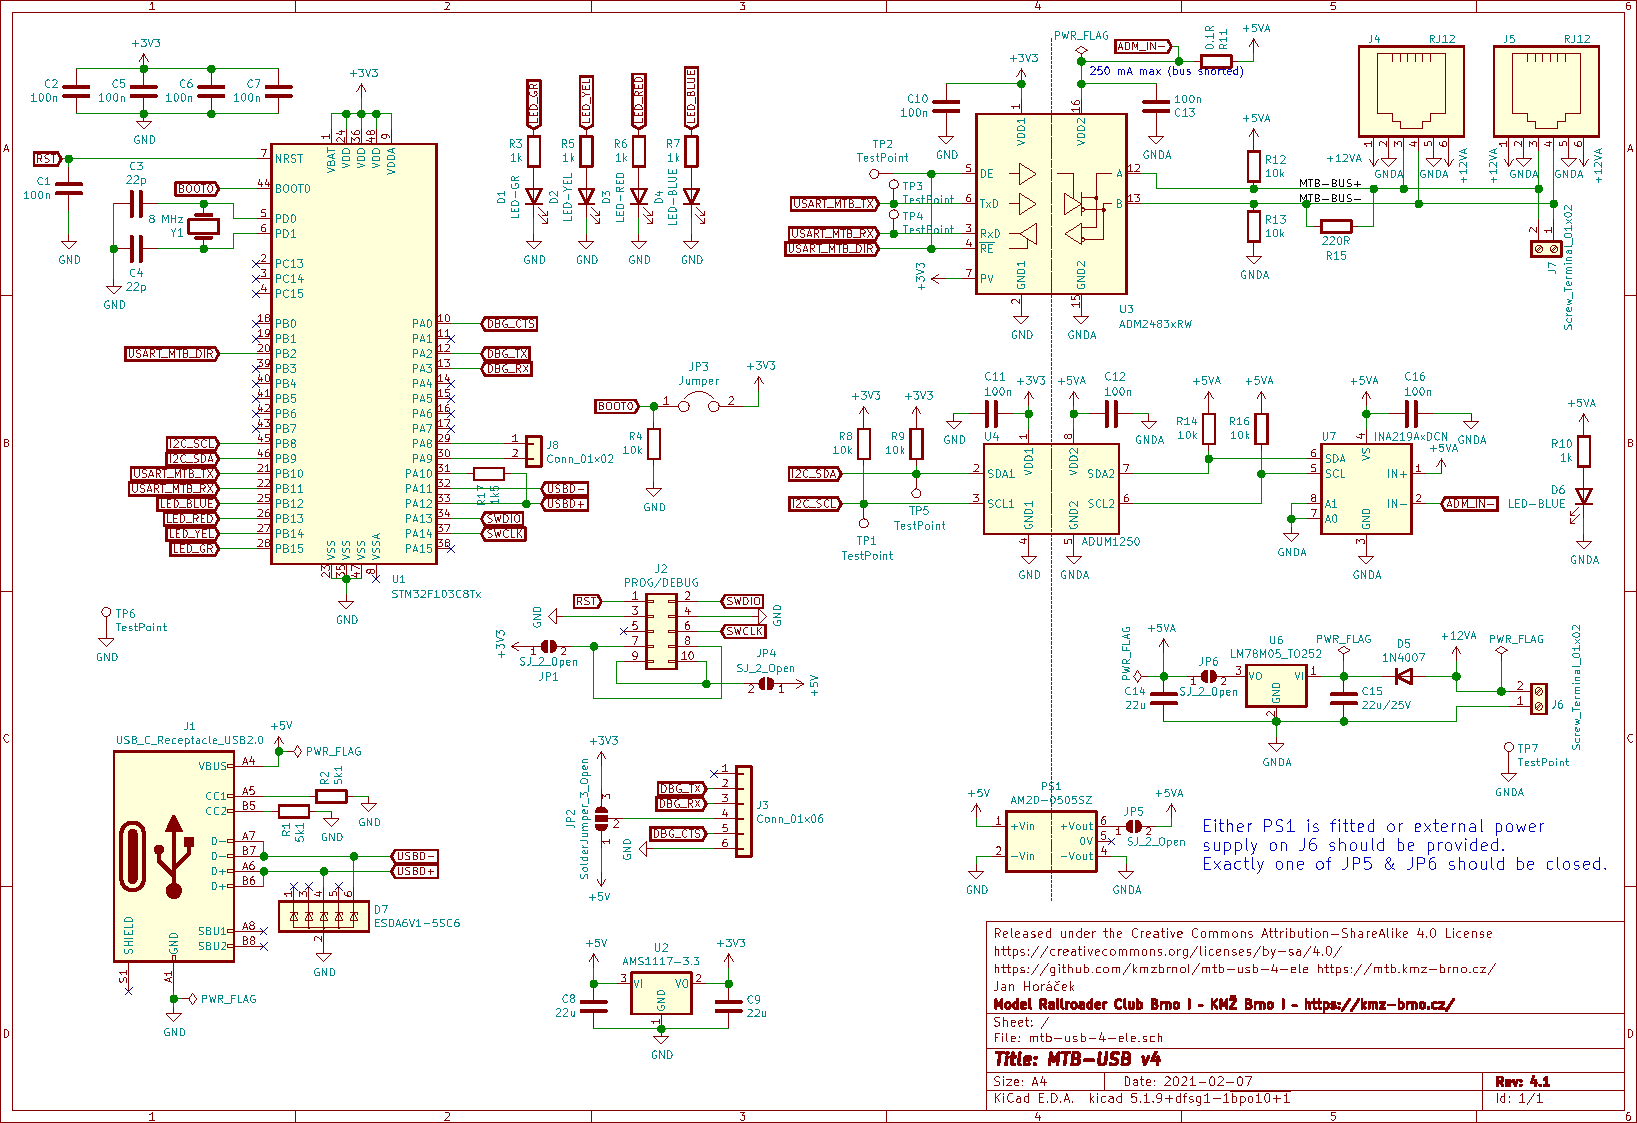
\includegraphics[angle=90,width=\textwidth]{data/mtb-usb-4-ele.pdf}
\caption{Schéma \gls{mtbusb} modulu.}
\label{fig:mtb-usb-sch}
\end{figure}

\begin{figure}[ht]
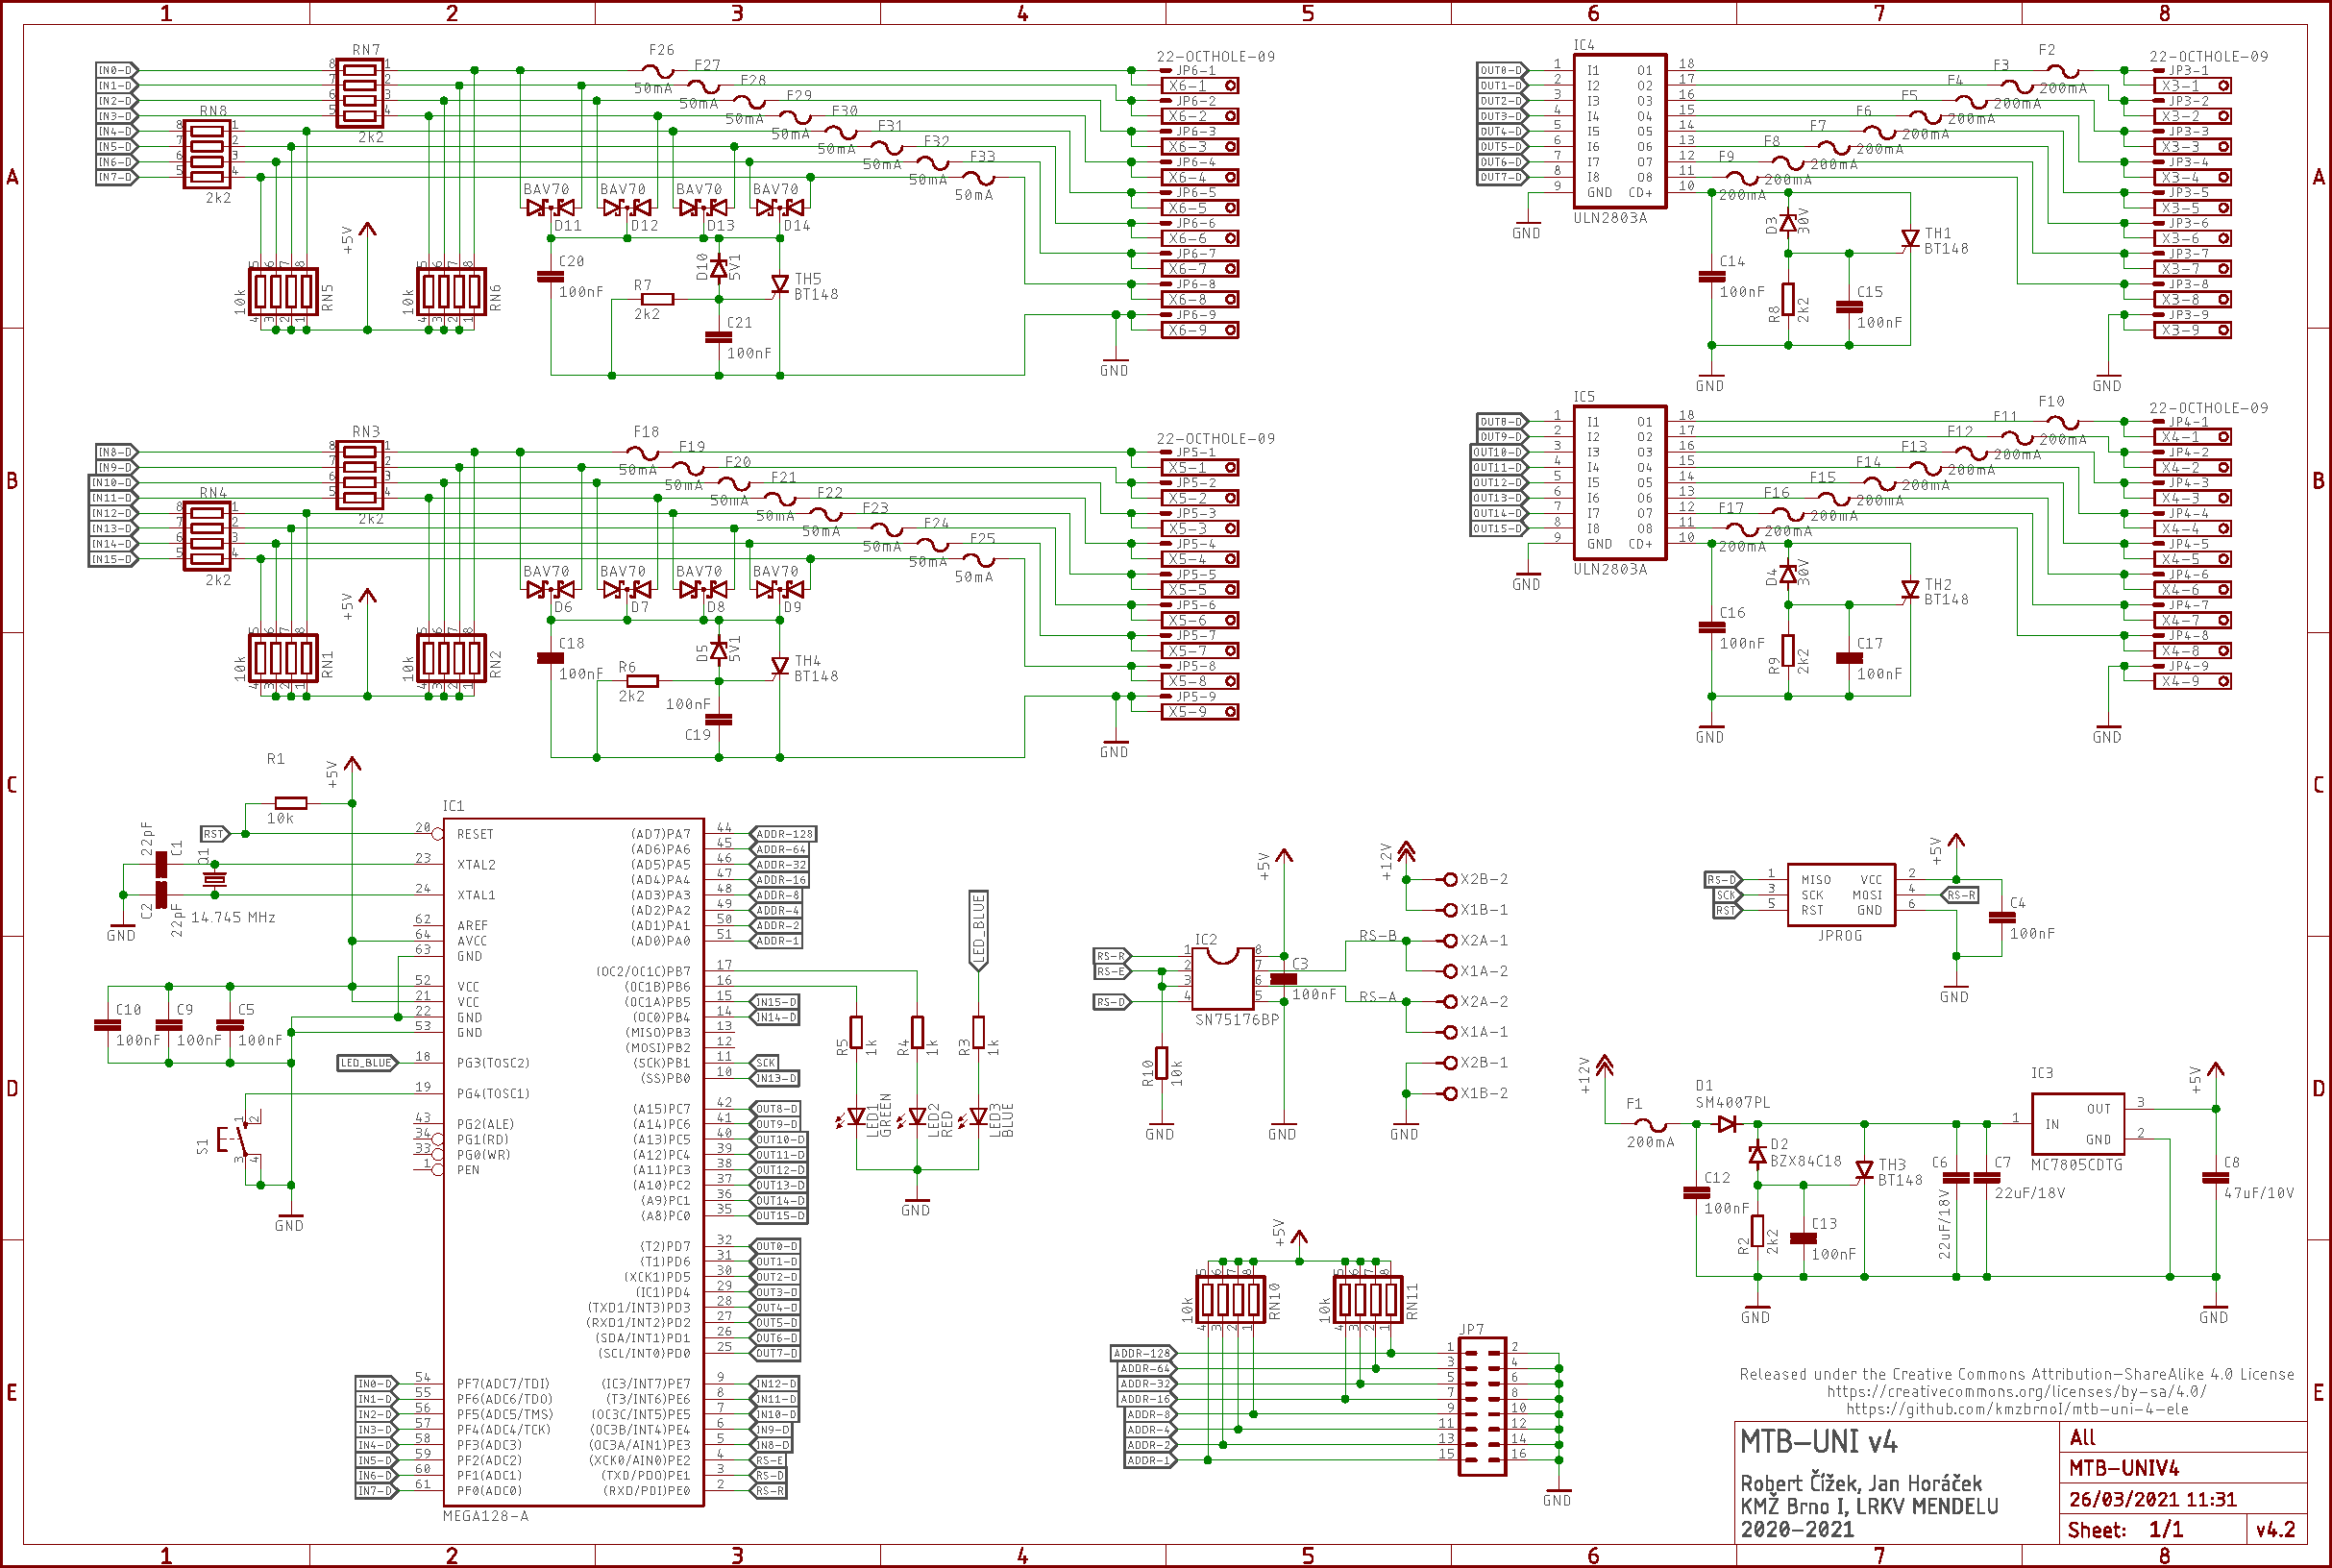
\includegraphics[angle=90,width=\textwidth]{data/mtb-uni-4-ele.pdf}
\caption{Schéma \gls{mtbuni} v4 modulu.}
\label{fig:mtb-uni-4-sch}
\end{figure}

\begin{figure}[ht]
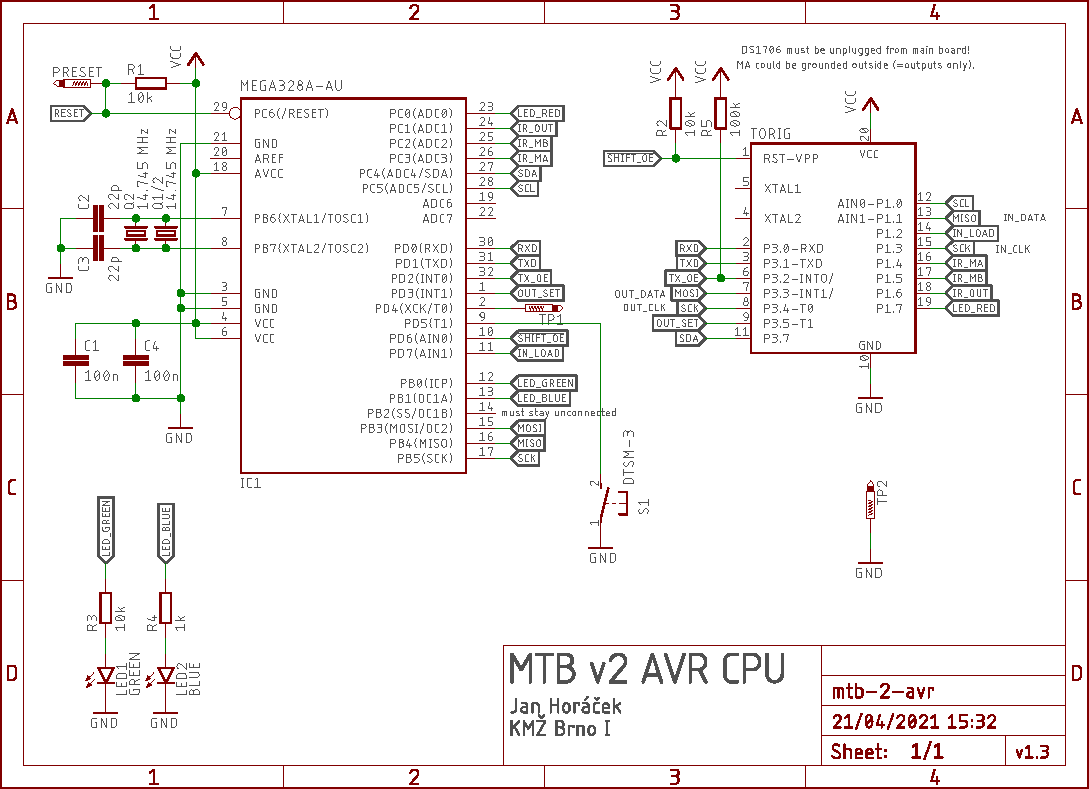
\includegraphics[angle=90,width=\textwidth]{data/mtb-2-avr-ele.pdf}
\caption{Schéma nástavné desky \textit{MTB-2-AVR}.}
\label{fig:mtb-uni-2-avr-sch}
\end{figure}

\begin{figure}[ht]
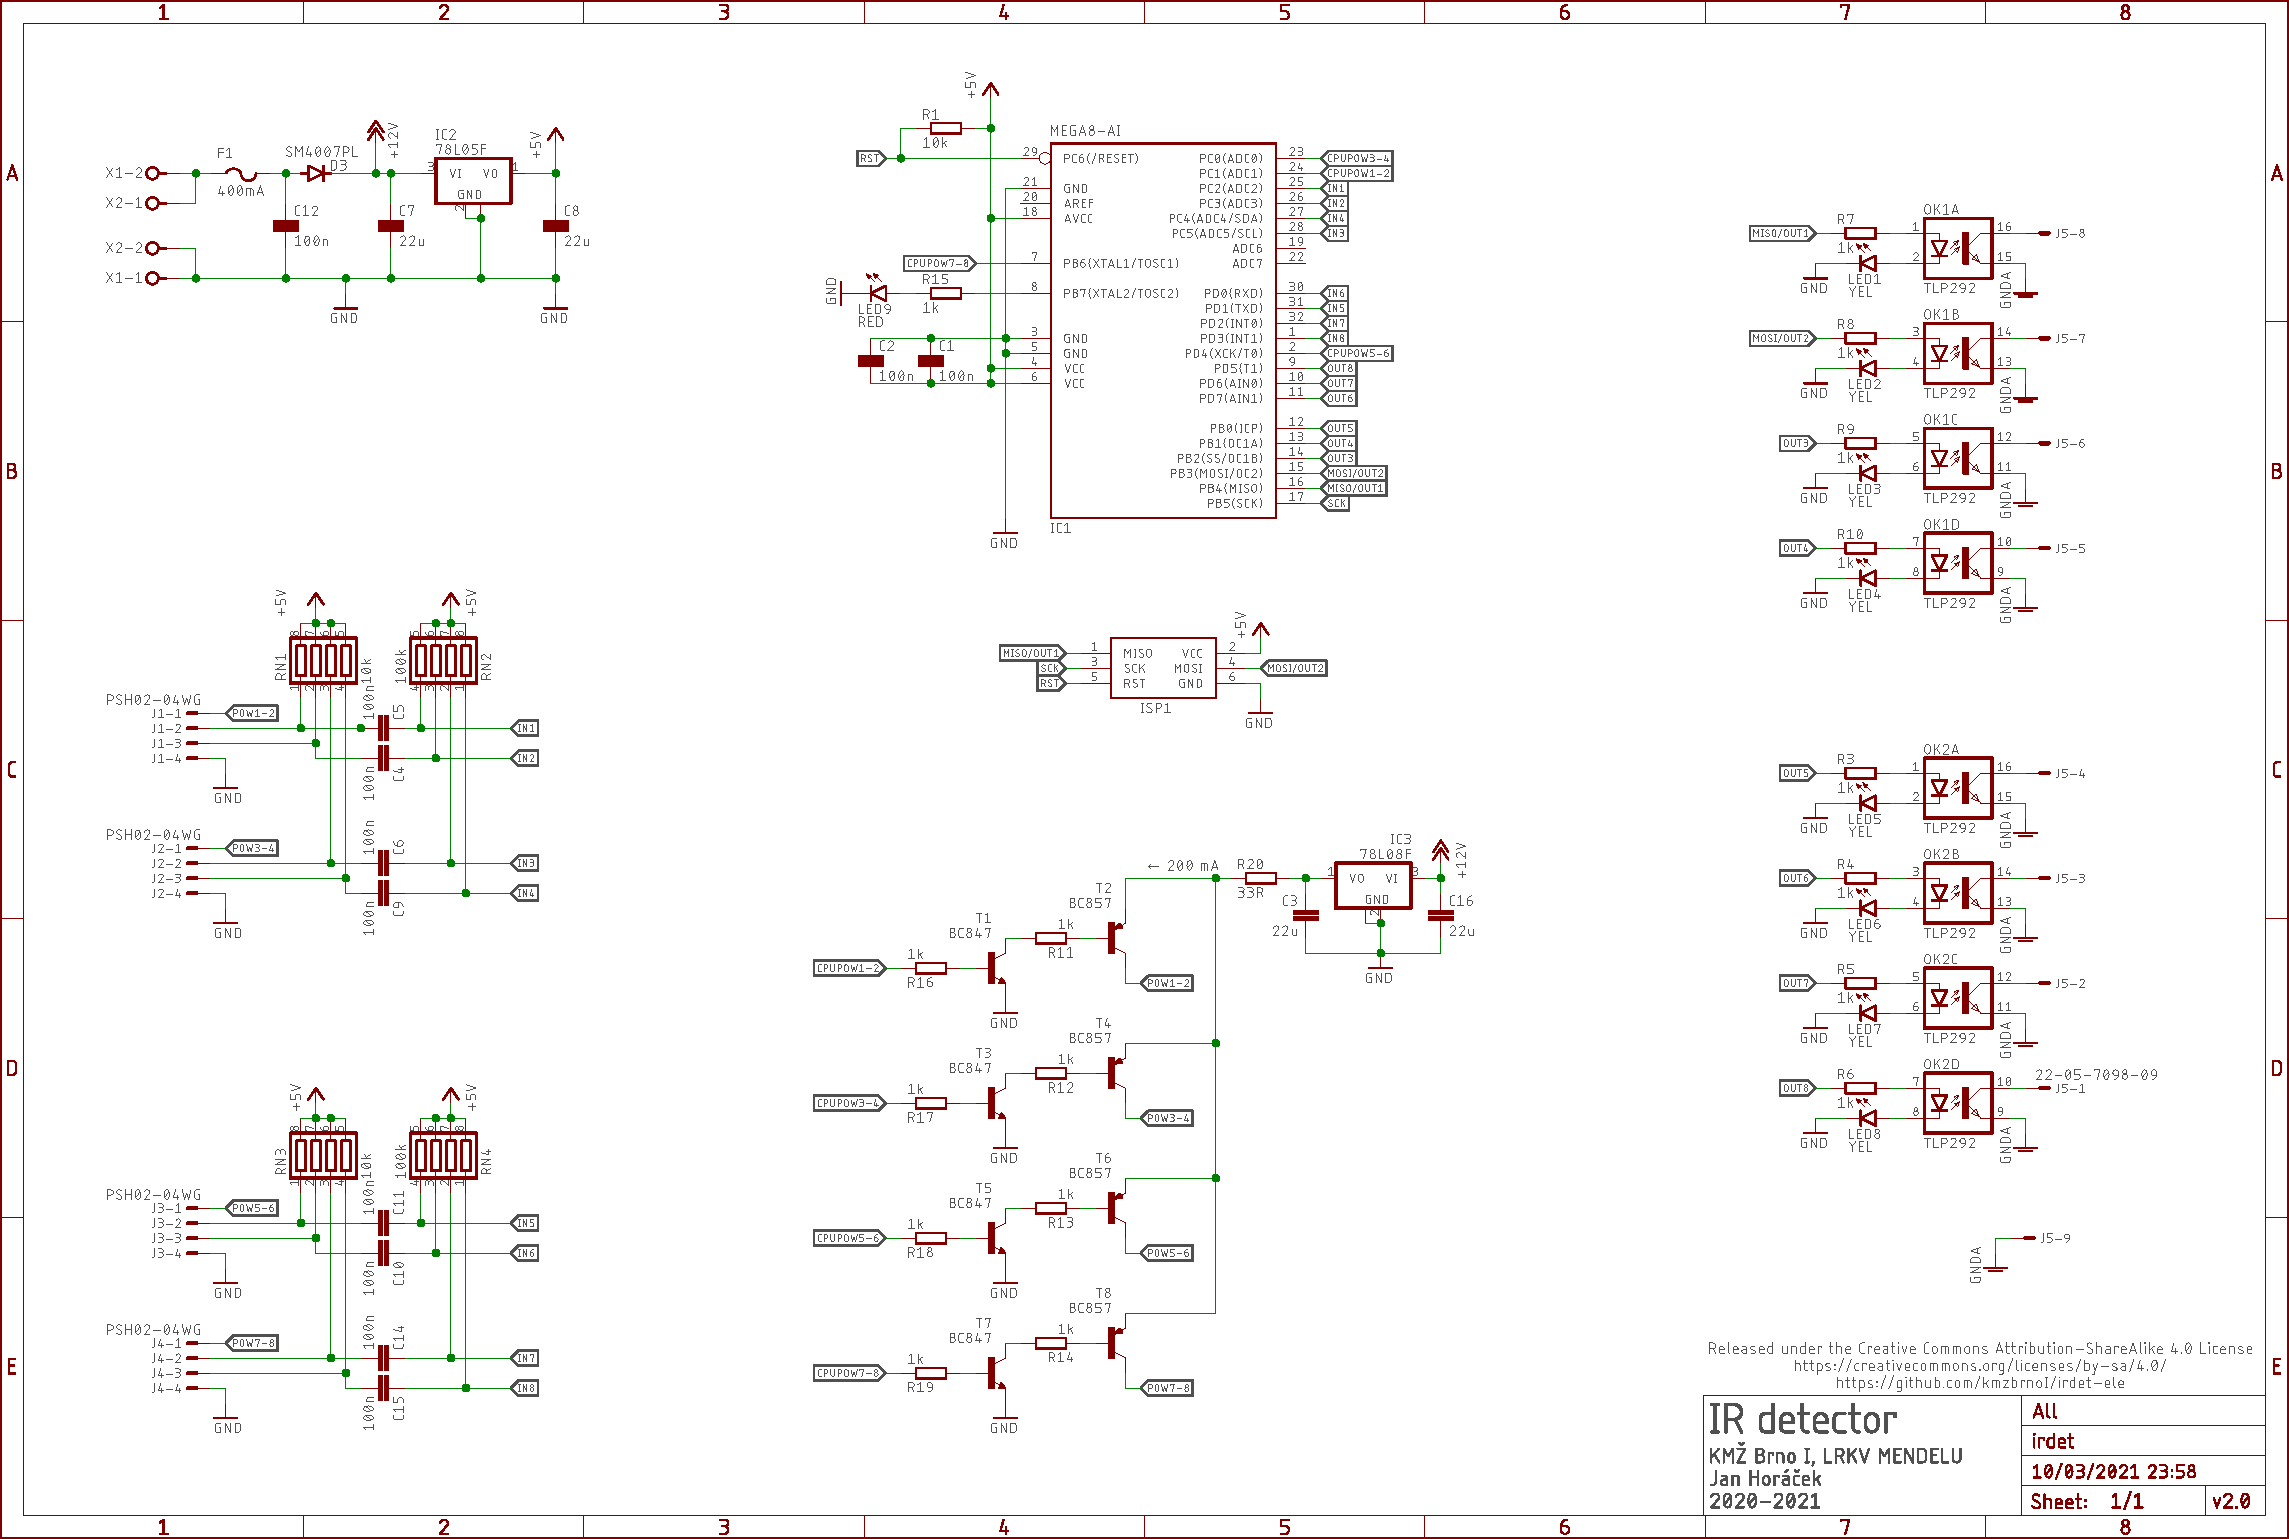
\includegraphics[angle=90,width=\textwidth]{data/irdet-ele.pdf}
\caption{Schéma desky \textit{IRdet}.}
\label{fig:irdet-sch}
\end{figure}


\end{document}
